\documentclass{article}
\usepackage[utf8]{inputenc}
\usepackage{array}
\usepackage{amsmath, mathtools}
\usepackage{graphicx}
\usepackage{empheq}
\usepackage{float}
\usepackage{listings}
\usepackage{hyperref}
\usepackage{parskip}
\hypersetup{
    colorlinks=true,
    linkcolor=blue,
    filecolor=magenta,
    urlcolor=cyan,
}

\DeclarePairedDelimiter{\ceil}{\lceil}{\rceil}

\usepackage{color}

%New colors defined below


%Code listing style named "mystyle"
\lstdefinestyle{mystyle}{
  basicstyle=\footnotesize\ttfamily,
  keywordstyle=\bf\ttfamily\color[rgb]{0,.3,.7},
  commentstyle=\color[rgb]{0.133,0.545,0.133},
  stringstyle={\color[rgb]{0.75,0.49,0.07}},
  breaklines=true,
  breakatwhitespace=true,
  breaklines=true,
  captionpos=b,
  keepspaces=true,
  numbers=left,
  numbersep=5pt,
  showspaces=false,
  showstringspaces=false,
  showtabs=false,
  tabsize=2,
  sensitive=true,
}

%"mystyle" code listing set
\lstset{style=mystyle}

% https://tex.stackexchange.com/questions/95838/how-to-write-a-perfect-equation-parameters-description
\newenvironment{conditions}[1][let:]
  {#1 \begin{tabular}[t]{>{$}l<{$} @{${}={}$} l}}
  {\end{tabular}\\[\belowdisplayskip]}


\title{Cassandra Availability with Virtual Nodes}
\author{
  Joseph Lynch\\
  \texttt{joe.e.lynch@gmail.com}
  \and
  Josh Snyder\\
  \texttt{josh@code406.com}
}

\begin{document}

\maketitle

\section{Introduction}
When Cassandra introduced vnodes in version 1.2, cluster operators made new tradeoffs
with respect to cluster maintainability and availability \cite{vnodes}. In particular,
clusters became easier to scale and operate, but they lost \textit{significant}
availability.

The main benefit of vnodes is that the variance of data size held by any one host
decreases and operators can easily change the number of hosts participating in a
cluster. In return, vnodes trade off availability. As we document in this report,
the availability cost of vnodes is quantifiable, and unavoidable. We present a model
of the availability of a single-datacenter Cassandra cluster under failures. We
attempt to furthermore predict, for a given cluster configuration, what availability
guarantees are feasible to give users of the database.

Based on our model, we conclude that the Cassandra default of 256 virtual nodes
per physical host is unwise, as it results in steadily rising chance of
unavailability as cluster size grows. This is antithetical to Cassandra's
design goal of fault-tolerance. We further use the model to argue for a middle
ground which both achieves the maintainability goals of multiple vnodes and
at the same time provides high fault tolerance.

If you are familiar with Cassandra internals, feel free to skip straight to
\hyperref[sec:problem]{Problem Statement} and \hyperref[sec:analysis]{Analysis}.

\section{Cassandra Background}
Data in Cassandra is distributed across the cluster hosts according to a
consistent hashing algorithm. All data has a partition key, which Cassandra
hashes to yield an integer bounded within the hash space. Each node in the
cluster takes responsibility for storing data along one or more contiguous
ranges of the hash space as decided by the replication strategies assigned
to the keyspaces on the cluster.

Cassandra clusters achieve fault-tolerance in the \texttt{SimpleStrategy}
and \\
\texttt{NetworkTopologyStrategy} replication strategies by storing multiple
copies of each piece of data. The quantity of copies (replication factor) is
configurable, but is typically an odd number, with three being most common.
Higher replication factors achieve greater fault-tolerance, at the cost of
increased storage requirements.

Hosts in a Cassandra cluster are assigned one or more tokens which represent
positions in a hash space created by the hashing function. Having more than
one token per physical host leads to ``virtual'' nodes. The start of each
range is variable, depending on the location of tokens held by other nodes
in the cluster. The space in the hash space between tokens are known as
\textit{token ranges} and are the basis of all data replication. Depending on
the keyspace replication strategy, and the placement of thes ``virtual'' nodes,
different physical hosts will be chosen to store data in a token range.
For example, to achieve a replication factor of two using a
\texttt{SimpleStrategy} Cassandra assigns two different physical nodes to
each token range, while with the \texttt{NetworkTopologyStrategy} Cassandra
assures that data is replicated to physical nodes across datacenters and
spread across racks as well. In all replication strategies, however, virtual
nodes add additional neighbors to physical hosts.

\section{Problem}
\label{sec:problem}

In Cassandra's data placement strategy, availability is only compromised under
a single host failure if at least one additional physical host that owns an
intersecting range fails before the first host's data can be recovered. Prior
attempts have been made to model Cassandra's failure modes \cite{dataloss},
but they often do not take into account the recovery aspect of Cassandra where
it automatically \footnote{Not exactly automatically, but with the right
\href{https://github.com/Netflix/Priam}{automation} it can be automatic}
streams lost data to new hosts. We approach the problem from a different
direction, opting instead to model outages as a combination of losing a single
node plus losing a neighboring node that owns an intersecting token range
before recovery finishes, causing \texttt{UnavailableExceptions} to clients
operating at \texttt{QUORUM} consistency levels. We do not care about the
proportion of the ring that is unavailable or for how long as any
unavailability is unacceptable to customers.

\section{Analysis}
\label{sec:analysis}
We conduct our analysis on a cluster with $R=3$. Under $R=3$, the failure of
two interdependent nodes leaves some token range with only a single active node.
The remaining node can continue to serve reads and writes, but \emph{cannot}
produce a quorum. We consider any lack of quorum, anywhere in the cluster, to
be an outage.

Before virtual nodes, a host in an $RF=3$ cluster would inter-depend on 4
other hosts: its two left-neighbors and two right-neighbors. If the cluster
is small enough, the same node may serve as both a left-neighbor and a
right-neighbor. For example on a cluster with three hosts, each node
inter-depends with two others, with four hosts each node has three
inter-dependents, and with five or more hosts each node has four
inter-dependents. When a host places 256 virtual nodes into the ring, each
vnode it places inter-depends with 2-4 other nodes.

By adding multiple token ranges to the responsibility of a single server,
virtual nodes increase the inter-dependency and decrease availability by
coupling physical nodes together, but they also theoretically increase the
speed that you can recover nodes \footnote{In our experience, at least with
Cassandra 2.x and 3.0.x, inbound streaming tops out at significantly under
line rate, but this simply makes this model conservative}.
For the purposes of this analysis:

\begin{conditions}
 n       &  number of hosts in the cluster \\
 \lambda &  average failure rate of hosts (1/interval) \\
 S       &  size of the dataset per host (MB) \\
 v       &  number of tokens per physical node \\
 R       &  replication factor (number of replicas per token) \\
 B_{inc} &  maximum incoming bandwidth of a joining physical node in (MB/s) \\
 B_{out} &  maximum outgoing bandwidth of a stream (MB/s) \\
\end{conditions}

$n$ and $S$ are details of a particular Cassandra deployment, $v$ and $B_{out}$
are configuration options in \texttt{cassandra.yaml}, $R$ is determined by the
keyspace replication strategy and $\lambda$ and $B_{inc}$ are determined by the
hardware Cassandra is deployed to ($B_{inc}$ is also impacted by how efficiently
Cassandra streams data, we add an arbitrary fudge factor for this later).

\subsection{Availability Model}

Crucial to the availability calculation is how quickly nodes can recover. The
longer a host takes to recover, the longer a second failure can occur and cause
an outage. We model this in eq. \ref{recovery} as a variant of the Birthday
Problem \cite{neighbors}. For each token, we choose a random $2 * (R - 1)$
replica hosts, those that proceed and those that come after the token on the
Cassandra ring. This is a \textit{conservative} estimate of how many neighbors
each additional token adds because actual Cassandra replication prohibits
duplicates \cite{replication}. We then make the model even more conservative by
assuming rack awareness, and that the number of racks equals $R$, which
eliminates $\frac{n}{R}$ nodes from being possible replicas.

This model presents a \textit{best case} for vnodes.

\begin{subequations} \label{recovery}
    \begin{align}
        k & = v * (2 * (R - 1)) \\ \label{recoverya}
        n_{p} & = n - \frac{n}{R} \\
        E[n_{neighbors}] & = n_{p} * [1 - (1-\frac{1}{n_{p}})^k] \label{recoveryc} \\
        speed & = \min(B_{inc}, E[n_{neighbors}] * B_{out}) \\
        E[T_{recovery}] & = \frac{S}{speed} \\
        E[T_{recovery}] & = \frac{S}{\min(B_{inc}, E[n_{neighbors}] * B_{out})}
    \end{align}
\end{subequations}

This is a very conservative model, but for cloud environments like where
Cassandra racks generally map 1:1 with availability zones this kind of
conservative model is reasonably accurate. The rest of \ref{recovery} follows
from dividing the per node dataset size by the maximum effective bandwidth to
a recovering node. This gives us what we dub the ``critical window''
where any neighbor failing will cause a token range to lose quorum.

From equation \ref{recovery} we can see that as $v$ increases, we get faster
streaming until we reach diminishing returns because we have saturated the
inbound network of the joining node. At that point additional streams do not
help speed recovery.

Now that we can model the expected recovery time, we begin the failure model by
assuming that hosts fail as independent Poisson processes with parameter
$\lambda$. Note that modeling host failures as a Poisson process represents a
``best case scenario'' for cluster availability: real-life computers are not so
polite that they fail in a manner completely uncorrelated with their peers.

Under such a model the inter-arrival time of host failures follows an
exponential distribution with parameter $\lambda$, and therefore once a single
host failure happens, we lose a second replica of an overlapping range before
the recovery finishes with probability:

\begin{subequations} \label{avail}
\begin{align}
        P(outage|failure) & = F(\tau; \lambda_{eff}) \\ \label{availa}
        P(outage|failure) & = 1 - e^{-\lambda_{eff} * \tau} \\ \label{availb}
        \tau & = E[T_{recovery}] \\ \label{availc}
        \lambda_{eff} & = E[n_{neighbors}] * \lambda \\ \label{availd}
        P(outage|failure) & = 1 - e^{- E[T_{recovery}] * E[n_{neighbors}] * \lambda}
\end{align}
\end{subequations}

Equation \ref{availa} follows from the CDF of an exponential distribution with
parameter $\lambda_{eff}$, and equation \ref{availb} and \ref{availc} follow
because we only care about failures during the recovery period of the
neighboring hosts (which form a combined Poisson process with effective
parameter $\lambda_{eff}$).

Now, if we model each host as a splitting Poisson process with parameter
$\lambda$ and splitting probability $P(outage|failure)$, then each node
forms an outage Poisson process with parameter $\lambda_{split} = \lambda * P(outage|failure)$. If we then join the $n$ such processes, we have
a resulting global Poisson process with parameter $\lambda_{global} =
\lambda_{split} * n$. This yields equation \ref{outage}, which models the
average number of outages over an interval $\tau$.

\begin{empheq}[box=\fbox]{align} \label{outage}
\begin{split}
    E[outages] & = \lambda_{global} \\
    & = (n * \lambda_{split}) \\
    & = (n * (\lambda * P(outage|failure))) \\
    & = (n * (\lambda * (1 - e^{-E[T_{recovery}] * E[n_{neighbors}] * \lambda_{s}})))
\end{split}
\end{empheq}

From this model we can see that availability is compromised by increasing the
number of nodes ($n$), increasing the failure rate of those nodes ($\lambda$),
increasing the number of tokens per node ($v$), or decreasing the streaming
bandwidth. To see how badly availability reacts with plausible default settings
on a 96 node cluster in a cloud environment with machine failure rate
$\lambda=\frac{25}{century}=\frac{0.25}{year}$.

\begin{conditions}
 n       &  96 \\
 \lambda &  25 $\frac{1}{century}$ (= 0.25 $\frac{1}{year}$ = 7.9e-9 $\frac{1}{s}$) \\
 v       &  256 \\
 R       &  3 \\
 S       &  307,200 (MB, 300 gigabyte) \\
 B_{inc} &  125 (MB/s, 1 gigabit) \\
 B_{out} &  25 (MB/s, 200 megabit) \\
\end{conditions}

We model this over a century because the probabilities of outage are so low in a
single cluster that in any reasonable time span, the most likely number of outages
is zero. To fairly compare the different configuration options, we model this
system for a century and find that, on average, we expect ~2.98 failures, or
equivalently ~0.03 per year:

\begin{equation}
    \begin{split}
    A & = 96 * 25 * (1 - e^{-E[T_{recovery}] * E[n_{neighbors}] * \lambda_{s}}) \\
    & = 96 * 25 * (1 - e^{-2457 * 64 * 7.927e-9}) \\
    & = 2.98
    \end{split}
\end{equation}

In the case with only 4 vnodes, the availability is much better with
only ~0.35 failures per century = ~0.0035 failures per year, a full 10x more
availability!

\begin{equation}
    \begin{split}
    A & = 96 * 25 * (1 - e^{-E[T_{recovery}] * E[n_{neighbors}] * \lambda_{s}} \\
    & = 96 * 25 * (1 - e^{-2457 * 7.5 * 7.927e-9}) \\
    & = 0.35
    \end{split}
\end{equation}


We can clearly see in Fig.\ref{fig:outages_small_vnodes} that small numbers of
vnodes do not appreciably change availability (due to the streaming benefits),
but as the number of vnodes gets large we rapidly lose large amounts of
availability until we level out after the number of vnodes passes the number of
nodes. In fact, for this particular $\lambda$, the median number of outages is
still zero until $v=5$.

\begin{figure}[h!]
    \centering
    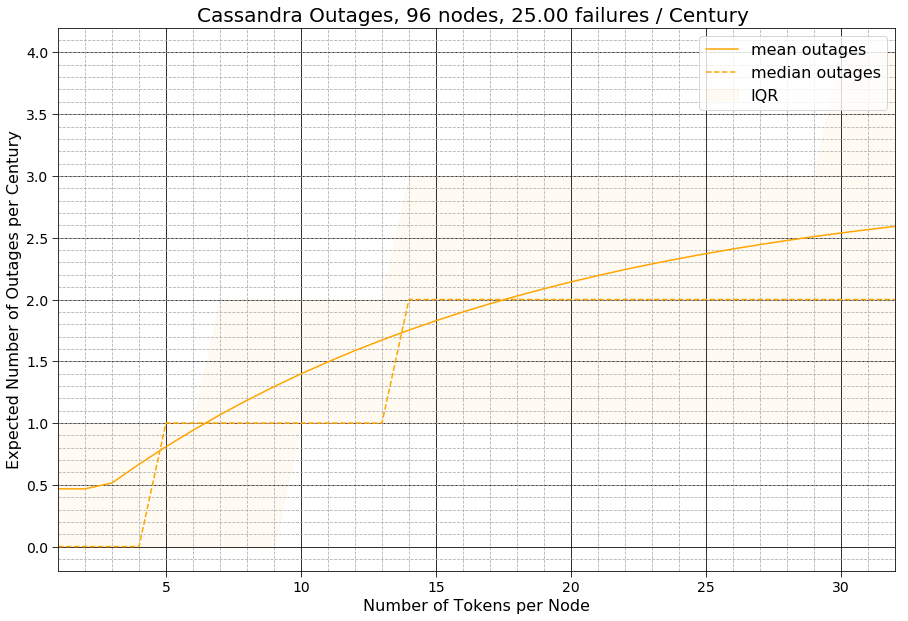
\includegraphics[width=1.0\textwidth]{images/outages_vnodes_small.png}
    \caption{Outages with Small Number of Tokens per Node}
    \label{fig:outages_small_vnodes}
\end{figure}

In Fig.\ref{fig:outages_all_vnodes} we see the effects of varying the failure
rate of machines, and observe that this has a significant impact on the
availability of a Cassandra cluster running with vnodes. In particular,
doubling the rate of machine failures can more than double the expected
number of outages. This makes intuitive sense because as we add more tokens
to each physical node, we are increasing the number of vulnerable replicas
during a single node failure. Rack placement helps a lot to limit the number
of potential replicas to only those residing in other racks, but it is not
enough to prevent likely outage with a high number of tokens per node.

\begin{figure}[h!]
    \centering
    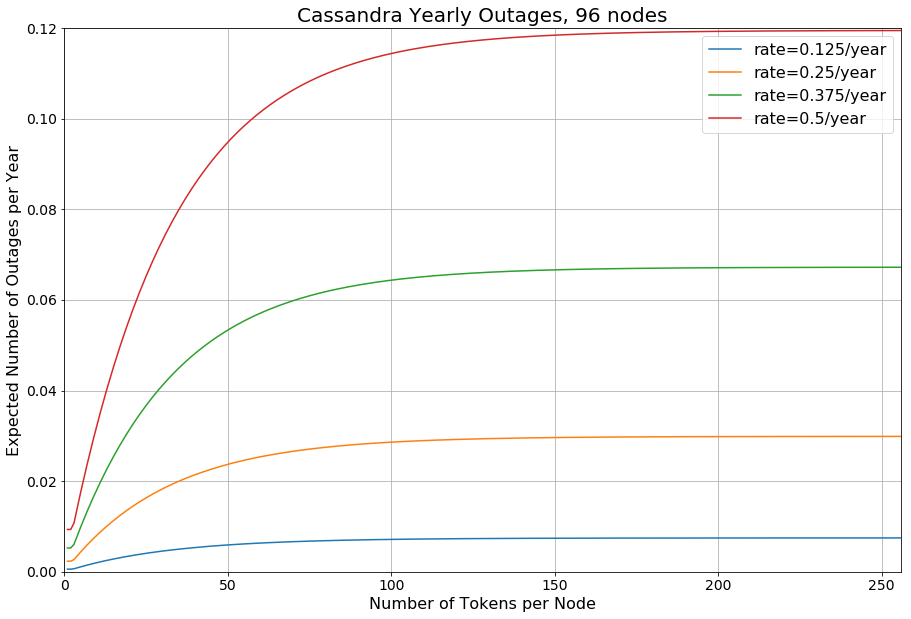
\includegraphics[width=1.0\textwidth]{images/outages_all_vnodes.png}
    \caption{Outages with Varying Tokens per Node}
    \label{fig:outages_all_vnodes}
\end{figure}

It is also interesting to note that as clusters get larger, holding everything
else constant, they become \textit{less available}. This intuitively makes
sense because as you increase the number of hosts significantly past RF,
you are creating more replicas that can fail and be vulnerable to a second
failure. Virtual nodes \textit{exacerbate} the problems for large clusters, causing significantly higher outages at large cluster sizes. This is shown in figure Fig. \ref{fig:outages_nodes}.

\begin{figure}[H]
    \centering
    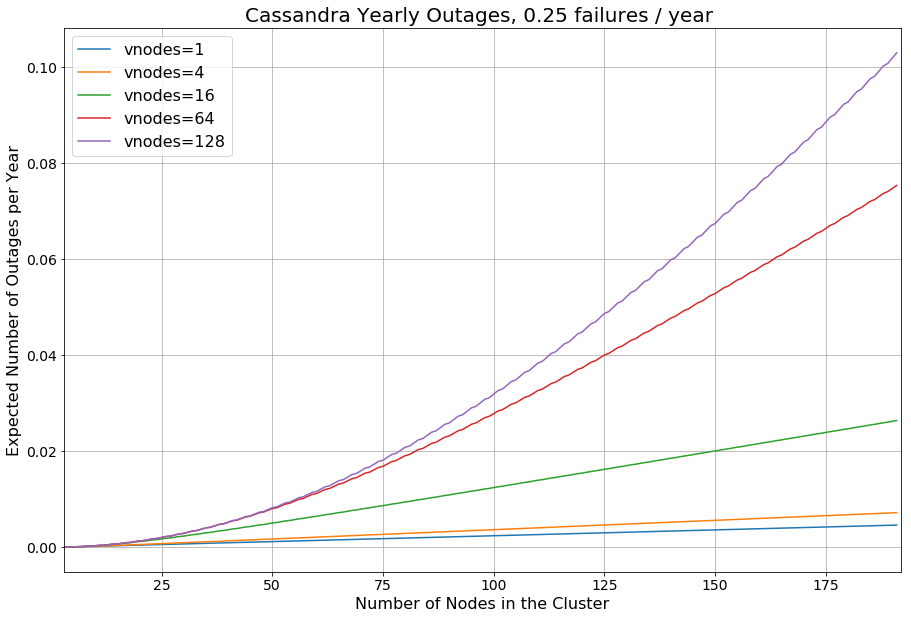
\includegraphics[width=1.0\textwidth]{images/outages_nodes.png}
    \caption{Outages with Varying Nodes in the Cluster}
    \label{fig:outages_nodes}
\end{figure}

However, as can be seen in Fig. \ref{fig:outages_nodes_small}, small clusters
($\leq16$ for \texttt{NetworkTopologyStrategy} or $\leq12$ for
\texttt{SimpleStrategy}) are not appreciably impacted by vnodes because all their
hosts are already neighbors with every possible host. As the cluster gets bigger,
small clusters have a constant number of neighbors, but large clusters gain more
and more neighbors, leading to 10-20x more risk of failure.

\begin{figure}[h]
    \centering
    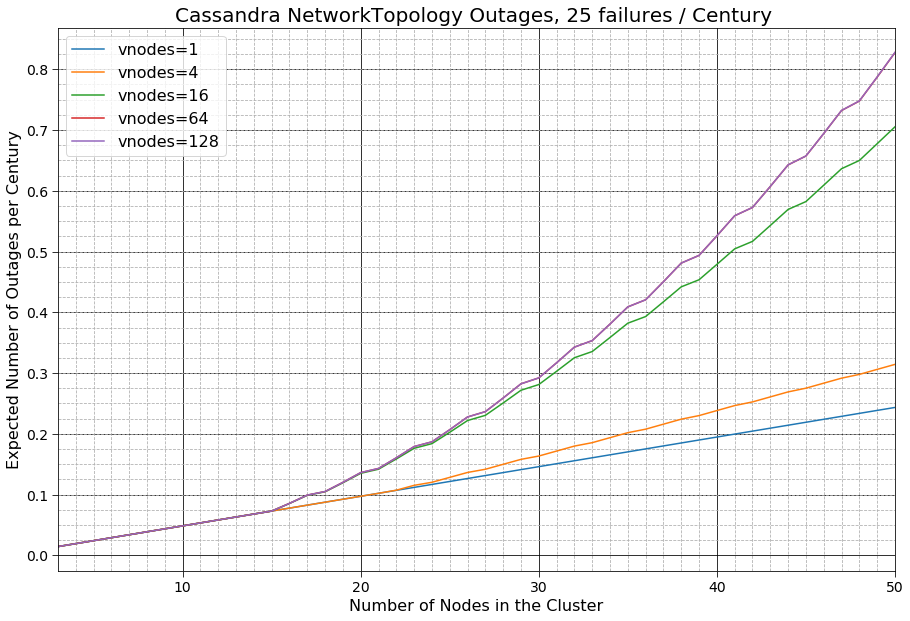
\includegraphics[width=1.0\textwidth]{images/outages_nodes_small.png}
    \caption{Outages with Varying Nodes in the Cluster}
    \label{fig:outages_nodes_small}
\end{figure}

The odd wiggle pattern you can see is because rack awareness has an integer
divide by 3, the \texttt{SimpleStrategy} graph is more smooth but also
less available in Fig \ref{fig:outages_nodes_small_simple}.

\begin{figure}[h]
    \centering
    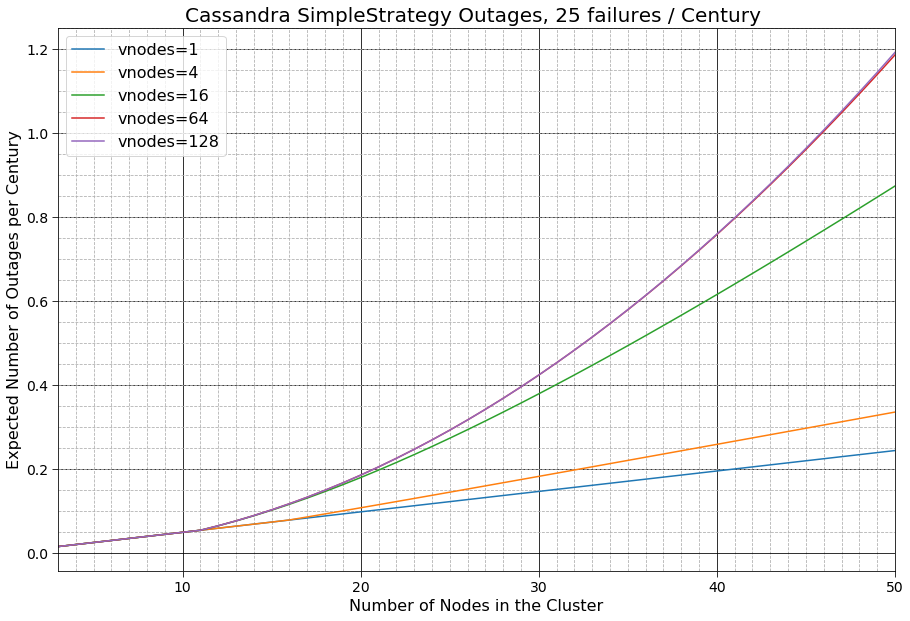
\includegraphics[width=1.0\textwidth]{images/outages_nodes_small_simple.png}
    \caption{Outages with Varying Nodes in the Cluster}
    \label{fig:outages_nodes_small_simple}
\end{figure}

Clearly, while 4 or 16 virtual nodes do not appreciably impact availability,
the default of 256 is quite unacceptable for large clusters.

\subsection{Virtual Nodes, the Benefits}

Having a number of tokens greater than 1 per physical nodes trades off
availability, but it gains data distribution and operations benefits. In
particular, a major problem pre-vnode was ``hot'' nodes, where one replica
may have significantly more data than other nodes. This was particularly
problematic when scaling up the cluster because in order to keep data evenly
distributed you had to effectively double the cluster. In particular to add
capacity to a cluster of size $n$ with $v$ vnodes you need proportionally fewer
new nodes $N$ to do so. Now that Cassandra token placement is reasonably good
at inserting new tokens where they are needed to balance the ring
\cite{tokenallocation}, we can model the number of nodes needed to scale up
with eq \ref{eq:scaling} as seen in figure \ref{fig:scaling}.

\begin{equation} \label{eq:scaling}
    N = \ceil*{\frac{n}{v}}
\end{equation}

As we can clearly see, as we add more vnodes we must add fewer
physical hosts to the cluster at a time in order to keep it balanced. While 1
token per host requires doubling, 16 tokens per host reduces this, naturally,
by a factor of 16, which is a \textit{significant} improvement. For a 96 host
cluster instead of needing 96 more machines, we can add in increments of 6. The
operational savings only get better as we add more tokens per host, until we
reach the size of the cluster at which point we reach diminishing returns.

\begin{figure}[H]
    \centering
    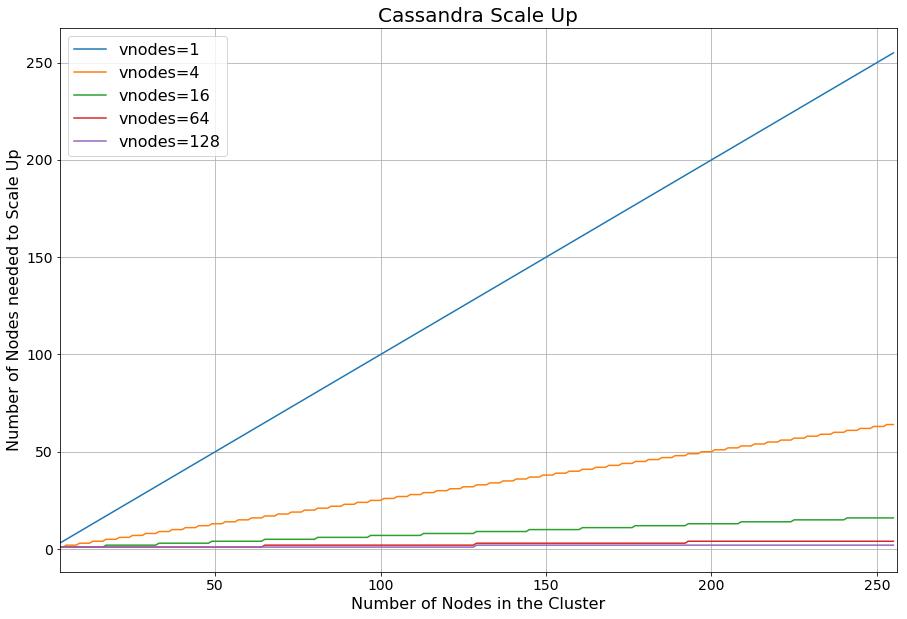
\includegraphics[width=1.0\textwidth]{images/scale_up.png}
    \caption{Nodes Required for Scaling Up}
    \label{fig:scaling}
\end{figure}

\section{Conclusion}

We have shown using a reasonable model that using a number of tokens per node
vnodes greater than the number of physical nodes in the cluster significantly
increases the expected outages, with default settings causing up to 10x more
frequent outages. This availability is traded away for more even distribution
of data and the ability to add fewer nodes and still maintain even distribution.
We believe, however, that a reasonable middle ground exists in the
\textbf{4-16 vnode range} where the streaming benefits mostly counteract the
additional risky neighbors and therefore the overall probability of outage is
still quite low. At the same time you can still scale up with
\textit{10x fewer} nodes than in the single token case. Changing the default
tokens per node in \texttt{cassandra.yaml} from 256 to 16 would yield
\textbf{10x higher availability} and still have \textbf{10x better scalability}
than single token clusters.

\begin{thebibliography}{9}

\bibitem{vnodes}
Brandon Williams: Virtual nodes in Cassandra 1.2
\\\texttt{https://www.datastax.com/dev/blog/virtual-nodes-in-cassandra-1-2}

\bibitem{karger}
Karger, et. al. Consistent Hashing and Random Trees: Distributed Caching Protocols for Relieving Hot Spots on the World Wide Web
\\\texttt{https://dl.acm.org/citation.cfm?id=258660}

\bibitem{dataloss}
Martin Kleppmann: The probability of data loss in large clusters
\\\texttt{https://martin.kleppmann.com/2017/01/26/data-loss-in-large-clusters.html}

\bibitem{replication}
Cassandra Data replication, \texttt{NetworkAwareTopologyStrategy}
\texttt{https://docs.datastax.com/en/cassandra/latest/cassandra/architecture/archDataDistributeReplication.html}

\bibitem{neighbors}
Kyle Siegrist: The Birthday Problem
\\\texttt{http://www.randomservices.org/random/urn/Birthday.html}

\bibitem{tokenallocation}
Branimir Lambov: New token allocation algorithm in Cassandra 3.0
\\\texttt{https://www.datastax.com/dev/blog/token-allocation-algorithm}



\end{thebibliography}


\section{Appendix}

Source code for all graphs is available on \href{https://github.com/jolynch/python_performance_toolkit/blob/master/notebooks/cassandra_availability/cassandra_availability.ipynb}{github} as well as reproduced below.
\begin{lstlisting}[language=Python]

# coding: utf-8

# In[2]:


from __future__ import print_function
import math
import matplotlib
import numpy as np
import matplotlib.pyplot as plt
import matplotlib.patches as mpatches
from scipy.stats import poisson

get_ipython().run_line_magic('matplotlib', 'inline')

# Boils down to "If I pick hosts 2 * (rf - 1) * vnode times, how many
# distinct hosts will I have in expectation". Note that this is a slightly
# optimistic estimate because Cassandra won't place two replicas of the
# same token on the same machine or rack, but this is close enough for
# the model
# This is a variant of the Birthday Problem where we are interested
# in the number of distinct values produced
# http://www.randomservices.org/random/urn/Birthday.html
def num_neighbors(n, v, rf, strategy="rack"):
    k = 2 * v * (rf - 1)
    if strategy == "rack":
        # As cassandra is rack aware, we assume #racks == #replicas
        # This is maybe a bad assumption for some datacenter deployments
        n = n - (n // rf)
    else:
        # SimpleStrategy
        n = n - 1
    estimate = (n * (1.0 - (1.0 - 1.0/n) ** k))
    return max(rf - 1, min(estimate, n))

def p_outage_given_failure(recovery_seconds, num_neighbors, rate_in_seconds):
    x = math.exp(-1 * recovery_seconds * num_neighbors * rate_in_seconds)
    return 1 - x

def global_rate(node_rate, nodes, split_probability):
    return node_rate * nodes * split_probability

def recovery_seconds(size, bw_in, bw_out, neighbors):
    return int(size / (min(bw_in, neighbors * bw_out)))

# Default model
nodes = 96
vnodes = 256
rf = 3
# 1000 gigabytes
node_dataset_mb = 300 * 1024
# MB/s
bw_in = 125
# MB/s, cassandra.yaml has 25MBPS as the default
# but most operators observe maybe half of that
bw_out = 25 / 2
strategy = 'rack'

year_seconds = 60.0*60*24*365
century_seconds = 100 * year_seconds

# Model machines that fail on average
# 25 times per century a.k.a 1 in 4 machines
# fails per year, or a machine fails every
# 4 years
arate = 25
arate_in_seconds = 25 / century_seconds


print("\nFailure Rate Variability")
print("Neighbors for {0} vnodes: {1:.3f}".format(1, num_neighbors(nodes, 1, rf)))
print("Neighbors for {0} vnodes: {1:.3f}".format(4, num_neighbors(nodes, 4, rf)))
print("Neighbors for {0} vnodes: {1:.3f}".format(16, num_neighbors(nodes, 16, rf)))

aneighbors = num_neighbors(nodes, vnodes, rf)
arecovery = recovery_seconds(node_dataset_mb, bw_in, bw_out, aneighbors)
print("Neighbors for {0} vnodes: {1:.3f}".format(vnodes, aneighbors))


def outage_stats(vnodes, failure_rate_per_century, num_nodes, rf, bw_in, bw_out, strategy='rack'):
    neighbors = num_neighbors(num_nodes, vnodes, rf, strategy)
    recovery_s = recovery_seconds(node_dataset_mb, bw_in, bw_out, neighbors)
    p_failure = p_outage_given_failure(
        recovery_s, neighbors, failure_rate_per_century / century_seconds)

    lmb = global_rate(failure_rate_per_century, num_nodes, p_failure)
    return (poisson.mean(lmb), poisson.interval(0.50, lmb), poisson.median(lmb))

# Returns outages _per century_
def compute_outage(vnodes, failure_rate_per_century, num_nodes, rf, bw_in, bw_out, strategy='rack'):
    return outage_stats(
        vnodes, failure_rate_per_century, num_nodes, rf, bw_in, bw_out, strategy
    )[0]

print("{0:<6} {1:<8} {2:<8} {3:<8} -> {4:<6}".format(
    "rate", "rec_s", "p_fail", "g_lmb", "outages"
))
for rate in (12.5, 25, 50, 100, 200):
    recovery_s = recovery_seconds(node_dataset_mb, bw_in, bw_out, aneighbors)
    p_failure = p_outage_given_failure(
        recovery_s, aneighbors, rate / century_seconds)
    gl = global_rate(rate, nodes, p_failure)
    p = "{0:6.2f} {1:6.2f} {2:8.6f} {3:8.4f} -> {4:6.6f}".format(
        rate, recovery_s, p_failure, gl, poisson.mean(gl)
    )
    print(p)


# In[3]:


plt.figure(figsize=(15,10))
plt.title("Cassandra Outages, {0} nodes".format(nodes), fontsize=20)
plt.ylabel("Expected Number of Outages per Century", fontsize=16)
plt.xlabel("Number of Tokens per Node", fontsize=16)
plt.xlim(1, 128)
plt.axvline(x=96, color='k', linestyle='--', label='cluster size={0}'.format(nodes))
plt.gca().grid(True, which='major', linestyle='-', color='k')
plt.gca().grid(True, which='minor', linestyle='--')
plt.gca().yaxis.set_minor_locator(matplotlib.ticker.AutoMinorLocator(4))
plt.gca().xaxis.set_minor_locator(matplotlib.ticker.AutoMinorLocator(4))
plt.tick_params(axis='both', which='major', labelsize=14, length=6)
plt.tick_params(axis='both', which='minor', length=0)

num_vnodes = range(1, 128)
rates = [12.5, 25, 37.5, 50]
for rate in rates:
    outages = []
    for vnode in num_vnodes:
        outages.append(compute_outage(vnode, rate, nodes, rf, bw_in, bw_out))
    print(outages[:3])
    plt.plot(num_vnodes, outages, label="rate={0}/century".format(rate))
plt.legend(fontsize=16)

outages = [outage_stats(v, arate, nodes, rf, bw_in, bw_out) for v in num_vnodes[:32]]
outage_mean = [o[0] for o in outages]
outage_lower = [o[1][0] for o in outages]
outage_upper = [o[1][1] for o in outages]
outage_median = [o[2] for o in outages]

plt.figure(figsize=(15,10))
plt.title(
    "Cassandra Outages, {0} nodes, {1:.2f} failures / Century ".format(
        nodes, arate), fontsize=20)
plt.ylabel("Expected Number of Outages per Century", fontsize=16)
plt.xlabel("Number of Tokens per Node", fontsize=16)
plt.xlim(1, 32)
plt.gca().grid(True, which='major', linestyle='-', color='k')
plt.gca().grid(True, which='minor', linestyle='--')
plt.gca().yaxis.set_minor_locator(matplotlib.ticker.AutoMinorLocator(5))
plt.gca().xaxis.set_minor_locator(matplotlib.ticker.AutoMinorLocator(5))
plt.tick_params(axis='both', which='major', labelsize=14, length=6)
plt.tick_params(axis='both', which='minor', length=0)
plt.plot(num_vnodes[:32], outage_mean, color='orange', label='mean outages')
plt.plot(num_vnodes[:32], outage_median, color='orange', label='median outages', linestyle='--')
plt.fill_between(num_vnodes[:32], outage_lower, outage_upper, color='orange', alpha=0.05, label='IQR')
plt.legend(fontsize=16)


# In[8]:


# Hold failures constant, vary size of cluster
plt.figure(figsize=(15,10))
plt.title(
    "Cassandra Outages, {1} failures / Century ".format(
        vnodes, arate), fontsize=20)
plt.ylabel("Expected Number of Outages per Century", fontsize=16)
plt.xlabel("Number of Nodes in the Cluster", fontsize=16)
plt.gca().grid(True, which='major', linestyle='-', color='k')
plt.gca().grid(True, which='minor', linestyle='--')
plt.gca().yaxis.set_minor_locator(matplotlib.ticker.AutoMinorLocator(5))
plt.gca().xaxis.set_minor_locator(matplotlib.ticker.AutoMinorLocator(5))
plt.tick_params(axis='both', which='major', labelsize=14, length=6)
plt.tick_params(axis='both', which='minor', length=0)

num_vnodes = (1, 4, 16, 64, 128)
num_nodes = range(3, 300)
lines = []
fills = []
for v in num_vnodes:
    outages = [outage_stats(v, arate, n, rf, bw_in, bw_out) for n in num_nodes]
    outages = [outage_stats(v, arate, n, rf, bw_in, bw_out) for n in num_nodes]
    outage_mean = [o[0] for o in outages]
    outage_lower = [o[1][0] for o in outages]
    outage_upper = [o[1][1] for o in outages]
    line, = plt.plot(num_nodes, outage_mean, label="vnodes={0}".format(v))
    lines.append(line)
    fill = plt.fill_between(
        num_nodes, outage_lower, outage_upper, alpha=0.1,
        label='vnodes={0} IQR'.format(v)
    )
    fills.append(fill)


plt.xlim(3, 300)
iqr_patch = mpatches.Patch(color='gray', label='IQR')
plt.legend(
    handles=lines + [iqr_patch], loc='upper left', fontsize=16
)

# Hold failures constant, vary size of cluster, NetworkTopologyStrategy
plt.figure(figsize=(15,10))
plt.title(
    "Cassandra NetworkTopology Outages, {0} failures / Century ".format(
        arate), fontsize=20)
plt.ylabel("Expected Number of Outages per Century", fontsize=16)
plt.xlabel("Number of Nodes in the Cluster", fontsize=16)
plt.gca().grid(True, which='major', linestyle='-', color='k')
plt.gca().grid(True, which='minor', linestyle='--')
plt.gca().yaxis.set_minor_locator(matplotlib.ticker.AutoMinorLocator(4))
plt.gca().xaxis.set_minor_locator(matplotlib.ticker.AutoMinorLocator(10))
plt.tick_params(axis='both', which='major', labelsize=14, length=6)
plt.tick_params(axis='both', which='minor', length=0)

num_vnodes = (1, 4, 16, 64, 128)
num_nodes = range(3, 51)
for v in num_vnodes:
    outages = [compute_outage(v, arate, n, rf, bw_in, bw_out, 'rack') for n in num_nodes]
    print(v, outages[:3])
    plt.plot(num_nodes, outages, label="vnodes={0}".format(v))

plt.xlim(3, 50)
plt.legend(fontsize=16)


# In[5]:


# Hold failures constant, vary size of cluster
plt.figure(figsize=(15,10))
plt.title(
    "Cassandra SimpleStrategy Outages, {0} failures / Century ".format(
        arate), fontsize=20)
plt.ylabel("Expected Number of Outages per Century", fontsize=16)
plt.xlabel("Number of Nodes in the Cluster", fontsize=16)
plt.gca().grid(True, which='major', linestyle='-', color='k')
plt.gca().grid(True, which='minor', linestyle='--')
plt.gca().yaxis.set_minor_locator(matplotlib.ticker.AutoMinorLocator(4))
plt.gca().xaxis.set_minor_locator(matplotlib.ticker.AutoMinorLocator(10))
plt.tick_params(axis='both', which='major', labelsize=14, length=6)
plt.tick_params(axis='both', which='minor', length=0)

num_vnodes = (1, 4, 16, 64, 128)
num_nodes = range(3, 51)
for v in num_vnodes:
    outages = [compute_outage(v, arate, n, rf, bw_in, bw_out, 'simple') for n in num_nodes]
    print(v, outages[:3])
    plt.plot(num_nodes, outages, label="vnodes={0}".format(v))

plt.xlim(3, 50)
plt.legend(fontsize=16)


# In[6]:


# Observe impact of vnodes on Scale Up Balancing
plt.figure(figsize=(15,10))
plt.title("Cassandra Scale Up",fontsize=20)
plt.ylabel("Number of Nodes needed to Scale Up", fontsize=16)
plt.xlabel("Number of Nodes in the Cluster", fontsize=16)
plt.gca().grid(True, which='major', linestyle='-', color='k')
plt.gca().grid(True, which='minor', linestyle='--')
plt.gca().yaxis.set_minor_locator(matplotlib.ticker.AutoMinorLocator(5))
plt.gca().xaxis.set_minor_locator(matplotlib.ticker.AutoMinorLocator(5))
plt.tick_params(axis='both', which='major', labelsize=14, length=6)
plt.tick_params(axis='both', which='minor', length=0)

num_vnodes = (1, 4, 16, 64, 128)
num_nodes = range(3, 256)
for v in num_vnodes:
    scale_up = [math.ceil(float(n) / v) for n in num_nodes]
    plt.plot(num_nodes, scale_up, label="vnodes={0}".format(v))

plt.xlim(3, 256)

plt.legend(fontsize=16)


# In[7]:


import itertools
import random
import sys

def simulate(l):
    return random.expovariate(l)

def offset(values, max_value=float("inf")):
    nvalues = values[:1] + [0] * (len(values) - 1)
    for i in range(1,len(values)):
        nvalues[i] = values[i] + nvalues[i-1]
    return [n for n in nvalues if n <= max_value]

def outage(o, f_i, t, neighbors):
    failures = 0
    neighbor_indices = range(0, len(o))
    neighbor_indices.remove(f_i)
    random.shuffle(neighbor_indices)
    for n in range(int(round(neighbors))):
        failures += near(o[neighbor_indices[n]], o[f_i], t)
    return failures

def near(a, b, t):
    failures = 0
    for i in a:
        for j in b:
            if j > i + t:
                break
            if j - i > 0 and j - i < t:
                failures += 1
    return failures

def run_simulate(l, neighbors, nodes):
    rs = []
    for r in range(5):
        o = [offset([simulate(l) for j in range(300)]) for i in range(nodes)]
        maxes = [x[-1] for x in o]
        m = max(maxes)
        outages_per_century = (
            sum([outage(o, i, arecovery / century_seconds, neighbors) for i in range(nodes)]) /
            m
        )
        print("Run {0} gave {1:.3f} outages/century".format(r, outages_per_century))
        rs.append(outages_per_century)
    print("Simulation outages/century: ", sum(rs) / len(rs))

def run_simulate_naive(l, neighbors, nodes):
    p_split = p_outage_given_failure(arecovery, aneighbors, l / century_seconds)
    l_split = l * p_split
    l_global = nodes * l_split
    print(p_split, l_global)
    rs = []
    for r in range(10):
        events = 1000
        o = offset([simulate(l_global) for j in range(events)])
        ##failure_years = [int(x/year) for x in o]
        num_centuries = max(o)
        rs.append(events / num_centuries)
    print("Simple simulation outages/century: ", sum(rs) / len(rs))


print(p_outage_given_failure(arecovery, num_neighbors(nodes, vnodes, rf), arate))
print(vnodes, arate, nodes, rf, bw_in, bw_out, arecovery, num_neighbors(nodes, vnodes, rf))
print("Predicted outages/century:", compute_outage(vnodes, arate, nodes, rf, bw_in, bw_out))
#run_simulate(arate, num_neighbors(nodes, vnodes, rf), nodes)
run_simulate_naive(arate, num_neighbors(nodes, vnodes, rf), nodes)
#run_simulate(arate, num_neighbors(nodes, vnodes, rf), nodes)

\end{lstlisting}

\end{document}
